\chapter{Hydroglaciological modelling of glacierized French alpine catchments}
\label{chap:discussion}

\begin{flushright}
\begin{small}
\textit{In the study of nature, as in the practice of art, it is not given to man to achieve the goal without leaving a trail of dead ends he had pursued.}\\ \\
Baron Louis Bernard Guyton de Morveau
\end{small}
\end{flushright}

\section{Introduction}

Glaciers supply water that supports ecosystems and human communities both nearby and far away from glaciers \citep{ipcc_climate_2018}. The strong climatic diversity of glacierized alpine catchments enables the storage of precipitation in the form of snow, firn and ice at high altitudes. This water storage is progressively released throughout the year during the warmest months, providing a more constant runoff than non-glacierized catchments. At the beginning of the melt season, snow provides important water resources downstream. Once most of the snow has melted, leaving bare glacier ice exposed, glaciers continue providing freshwater resources, ensuring an uninterrupted runoff throughout the melt season \citep{huss_toward_2017}. This role of glaciers as late summer buffers is currently being challenged by anthropogenic climate change. Glacier retreat in the European Alps is transforming the hydrological regime of high-mountain catchments, with potential environmental and social impacts \citep{zekollari_modelling_2019}. In the French Alps, the local population have a strong dependency on water resources, using them for the ski business \citep{spandre_winter_2019}, hydropower generation and domestic use. The regional socioeconomic model is built around mountain tourism, with a strong dependency on the cryosphere, both as a tourism attraction \citep{schut_sport_2013} and as an electricity generation source \citep{schaefli_role_2019}. Moreover, late summer runoff from glaciers provides reliable water resources for domestic use, industries and agriculture. This decrease in glacier freshwater contributions has ecological impacts as well, decreasing biodiversity in glacier-fed rivers \citep{cauvy-fraunie_global_2019} and in humid areas that no longer receive runoff during the warmest period of the year \citep{carlson_monitoring_2020}. Glaciers provide cold water resources that help regulate the temperature, flow regimes, sediment concentration and nutrient supply of mountain streams \citep{huss_toward_2017}. These cold waters are essential to some specialized species, whose survival will be challenged by glacier retreat \citep{lencioni_glacial_2018, cauvy-fraunie_global_2019}.  Alternatively, these changing streams can be quickly colonized by aquatic communities adapted to higher water temperatures, increasing competition between species  \citep{robinson_ecosystem_2014}. Anticipating these future hydrological changes is of paramount importance in order to correctly adapt and manage future water social and environmental needs. 

Hydrological models can provide answers to these questions, predicting the hydrological evolution under of different future climate scenarios. In France, multiple hydrological models are being developed and used for research and operational purposes. The lumped GR rainfall-runoff models, coupled with the CemaNeigne snow component \citep{coron_suite_2017}, use a simplified modelling approach with catchment-scale representations of the transformation of precipitation into discharge. CROCUS-ISBA-MODCOU \citep{etchevers_simulation_2001} is coupled model, combining a soil-vegetation-atmosphere transfer scheme (ISBA), a one-dimensional snow model (CROCUS) and a macroscale hydrological model (MODCOU) developed by Météo-France. The MORDOR model \citep{paquet_evolution_2004}, developed by Électricité de France (EDF), is a hydrological operational model used to forecast runoff in mountain catchments in France. It is actively being used to anticipate changes in hydropower production, both for short and long term periods. The GSM-Socont model \citep{schaefli_conceptual_2005}, is a Swiss semi-distributed model used to simulate glacierized catchments. It has been recently applied to perform projections of the Arve watershed in the Mont-Blanc massif through the 21${st}$ century \citep{laurent_impact_2020}. Out of all these models, only the GSM model include a dynamic representation of glaciers (VERIFY FOR MORDOR). The vast majority of hydrological models have a very simplified representation of glaciers, including them as static ice reservoirs. Such a representation is problematic in the current context of glacier retreat, neglecting future changes in hydrological regimes driven by glaciers. 

This static representation of glaciers is also found in the J2K hydrological model \citep{krause_quantifying_2002}, developed at the University of Jena (Germany). J2K is a semi-distributed open-source model, based Hydrological Response Units (HRUs), homogeneous spatial units in terms of hydrological processes. It allows the representation of multiple physical processes, land use covers, pedology, geology and topography. Moreover, the representation of multiple anthropogenic water uses, such as agriculture or dams can be taken into account into the model.  J2K is being used by a large community of hydrologists, both in France and internationally, for a wide variety of geographical configurations \citep{krause_quantifying_2002, nepal_understanding_2014, braud_j2000-rhone_2017}. J2K has already been applied to glacierized catchments in the Himalayas \citep{nepal_understanding_2014}, but simulations have only been performed for past periods, keeping the glacier surface area constant in time. In this chapter, I present a new glacier module for J2K, including a dynamic representation of glaciers. We introduce and validate this new implementation in a partially-glacierized alpine catchment in the French Alps: the Arvan catchment in the Grandes Rousses massif. By introducing glacier evolution in a hydrological model, we aim at improving hydrological projections of glacierized catchments, in order to assess the impacts of these changes on communities living in glacier-fed streams. This objective is driven by the BERGER project, which combines the hydroglaciological modelling efforts of my work with an ecological study on the impacts and adaptation of glacier retreat on aquatic communities in the French Alps.

\section{Methods}

\subsection{Study area}

The Arvan catchment (Fig. \ref{hydro:fig1}) is a partially glacierized alpine catchment, situated in the Grandes Rousses massif, between 1368 and 3373 m.a.s.l. It includes the Saint Sorlin glacier (2.069 km$^{2}$ in 2015), being the glacier with the second longest mass balance observation series in France (1957-present). Two villages are located within the catchment: Saint-Sorlin-d'Arves and Saint-Jean-d'Arves, with the latter including runoff measurements for the 2000-2016 period. This station measured an average interannual runoff of 1.864 m$^{3}$/s, with 10\% of temporal gaps for this period (Fig. \ref{hydro:fig1}). This study site has been chosen due to its wealth of data, providing an excellent testbed to validate the modelling approach.

\begin{sidewaysfigure}[ht]
\centering
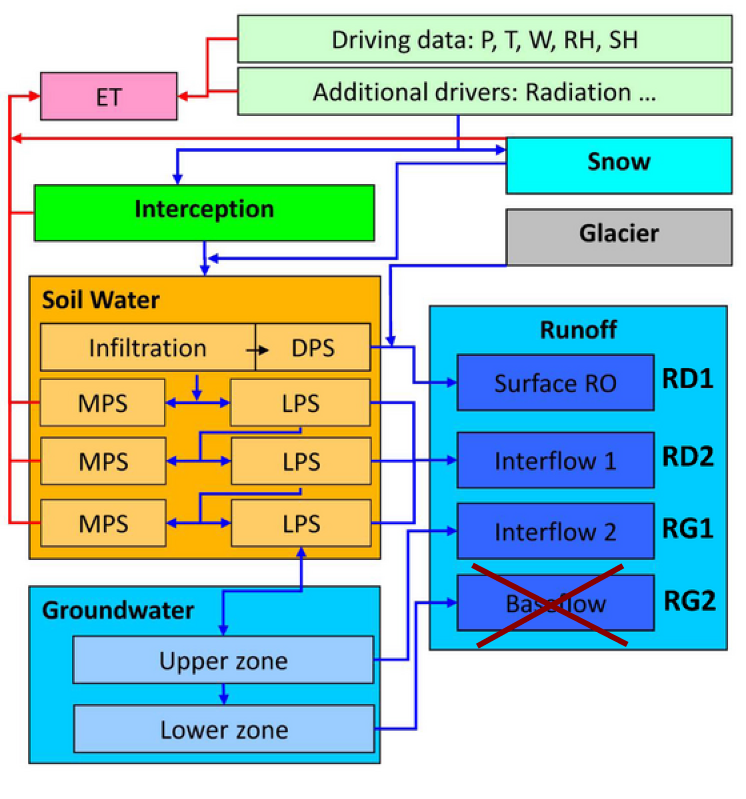
\includegraphics[width=23cm]{Figures/hydro/Figure_1.png}
\captionsetup{justification=centering}
\caption{Description of the Arvan catchment, based on hydrological data observed at the Saint-Jean-d'Arves (La Vilette) station. 
\textit{Figure from the HYDRO team from INRAE Antony}.}
\label{hydro:fig1}
\end{sidewaysfigure}

\subsection{Data}

The J2K hydrological model is forced with climate data coming from the SPAZM method \citep{gottardi_statistical_2012}. SPAZM is a statistical method to interpolate meteorological data, particularly precipitation, in mountain areas. This interpolation is based on an observational network, taking into account the local orography and the main atmospheric patterns in the French Alps bringing precipitation. With a resolution of 1 km$^{2}$, this dataset is well adapted to representing the complex meteorological conditions of a glacierized alpine catchment. 

\subsection{The J2K hydrological model}

\section{Results}

\section{Discussion and conclusions}


